%%%%%%%%%%%%%%%%%%%% author.tex %%%%%%%%%%%%%%%%%%%%%%%%%%%%%%%%%%%
%
% template for Encyclopedia articles
%
%%%%%%%%%%%%%%%% Springer %%%%%%%%%%%%%%%%%%%%%%%%%%%%%%%%%%


% RECOMMENDED %%%%%%%%%%%%%%%%%%%%%%%%%%%%%%%%%%%%%%%%%%%%%%%%%%%
%\documentclass[graybox, natbib, nosecnum, twocolumn]{svmult}
\documentclass{svjour3}
\usepackage[english]{babel}
\usepackage[utf8x]{inputenc}
\usepackage[T1]{fontenc}

%% Sets page size and margins
\usepackage[a4paper,top=3cm,bottom=2cm,left=3cm,right=3cm,marginparwidth=1.75cm]{geometry}

%% Useful packages
\usepackage{amsmath}
\usepackage{graphicx}
\usepackage[colorinlistoftodos]{todonotes}
\usepackage[colorlinks=true, allcolors=blue]{hyperref}

%%%%%%%%%%%%%%%%%%%%%%%%%%%%%%%%%%%%%%%%%%%%%%%%%%%%%%%%%%%%%%%%%%%%%%%%%%%%%%%%%%%%%%%%%

\begin{document}

\title{Historical Graph Data Management}
% Use \titlerunning{Short Title} for an abbreviated version of
% your contribution title if the original one is too long
\author{Udayan Khurana and Amol Deshpande}
% Use \authorrunning{Short Title} for an abbreviated version of
% your contribution title if the original one is too long
\institute{Udayan Khurana
		\at IBM Research AI, TJ Watson Research Center, Yorktown Heights New York NY, USA \\\email{ukhurana@us.ibm.com}
		\and
		Amol Deshpande
		\at Computer Science Department, University of Maryland, College Park MD, USA \\\email{amol@cs.umd.edu}
		}
%
% Use the package "url.sty" to avoid
% problems with special characters
% used in your e-mail or web address
%
\maketitle

\begin{abstract}
%Your abstract.
%\end{abstract}

%\section{Introduction}
Real world graphs evolve over time, with continuous addition and removal of vertices and edges, as well as frequent change in their attributes. Some examples of such graphs are -- phone-call graphs generated by telecommunication service providers, message graphs from social networking sites, and mention-activity graphs formed by Twitter users mentioning one another in their tweets, and so on.
For decades, the work in graph analytics was restricted to a static perspective of the graph. Analysis such as finding important (central) entities in a network, groups (clusters) of similar entities, observing graph density, diameter and several other attributes have been well studied in the context of static graph snapshots. 
In recent years, however, we have witnessed an increasing abundance of timestamped observational data describing
various types of temporal information networks, including social networks, biological networks,
citation networks, financial transaction networks, communication networks, to
name a few. This has fueled an interest in performing richer analysis of graphs, along a temporal dimension. Analysis of history of a graph presents fascinating insights into the underlying phenomena that produced the graph. 
However, the traditional network data management systems provide inadequate support for such analyses. We present a summary of recent advances in the field of historical graph data management. They involve, compact storage of large graph histories, efficient retrieval of temporal subgraphs, and effective interfaces for expressing historical graph queries are essential for enabling temporal graph analytics.  
\end{abstract}

\section{Overview}
In recent years, several works have designed analytical models that capture network evolution, with a focus on
social networks and the Web~\cite{LeskovecKF07,Kumar:2006:SEO:1150402.1150476}. Studies analyze how communities evolve~\cite{tang2008community}, identifying key individuals,
and locating hidden groups in dynamic networks~\cite{tantipathananandh2007framework}, also characterizing the complex behavioral patterns 
of individuals and communities over time~\cite{Asur2009}.
%present a framework that focuses on identifying communities and understanding how they change over time.
%Tang et al.~\cite{tang2008community} and Greene et al.~\cite{Greene2010} 
%address the problem of community evolution in
%dynamic networks.
%McCulloh and Carley~\cite{McCulloh2008} present techniques for social change detection.
%Asur et al.~\cite{Asur2009} present a framework for characterizing the complex behavioral patterns
%of individuals and communities over time. %Biologists share on predicting historical events leading to a 
%known biological network (e.g.,~\cite{10.1371/journal.pcbi.1001119})
Biologists are interested in discovering historical events leading to a 
known state of a biological network (e.g.,~\cite{10.1371/journal.pcbi.1001119}).
%Evolution of shortest paths in dynamic
%graphs has been studied by Huo et al.~\cite{huo2014efficient}, Ren et al.~\cite{RenEvolvGraph11},
%and Xuan et al.~\cite{xuan2003computing}. 
Change in page rank~\cite{bahmani2010fast}, change in centrality of vertices, path lengths of vertex pairs,
etc.~\cite{pan2011path}, shortest paths evolution~\cite{RenEvolvGraph11}, and such, provide useful analytical algorithms for changing graphs.
%Barrat et al.~\cite{barrat2008dynamical}, provide a good reference for studying several dynamic processes modeled over graphs. 
Historical or temporal analyses on graphs span a variety of tasks that vary in the analytical quantity of interest, as well as the scope of the graph locality and time-duration being analyzed. 
Figure~\ref{fig:et} provides a classification on those lines and lists a few examples of graph retrieval and analysis tasks.
A more exhaustive taxonomy of temporal tasks is provided by Ahn et al.~\cite{ahn2014task}.
%Holme et al.~\cite{holme2012temporal} provide a description of several networks from different domains that 
%are temporal or dynamic in nature. 

Typical graph data management systems that are based on static graphs, do not provide sufficient support for the analytical tasks described above. This is due to a fundamental lack in the modeling of the {\em change} of information. If performed using the conventional graph systems, such tasks become too expensive in storage costs, memory requirements, or execution time, and are often unfriendly or infeasible for an analyst to even express in the first place. 
The frequent change of a temporal graph also poses a significant challenge to algorithm design, because the overwhelming majority of graph algorithms assume static graph structures. One would have to design special algorithms for each application to accommodate the dynamic aspects of graphs. To support general-purpose computations, most of the emerging temporal graph systems adopt a strategy to separate graph updates from graph computation. More specifically, although updates are continually applied to a temporal graph, graph computation is only performed on a sequence of successive \emph{static} views of the temporal graph. For simplicity, most systems adopt a \emph{discretized-time} approach, so that time domain is set of natural numbers, i.e., $t\in \mathcal{N}$. 
As per the terminology of temporal relational databases, this discussion considers {\em valid time} (against {\em transaction time}) as the underlying temporal dimension for historical analyses. Valid time denotes the time
period during which a fact is true with respect to the real world. Transaction time is the time
when a fact is stored in the database. 
It is worth noting that there is a related but orthogonal body of work which we do not touch in this chapter. It deals with the need to do {\em real-time analytics on the streaming data} as it is being generated; here the scope of the analysis typically only includes the latest snapshot or the snapshots from a recent window. The key challenge there is to be able to deal with the high rate at which the data is often generated.

\begin{figure}
\centering
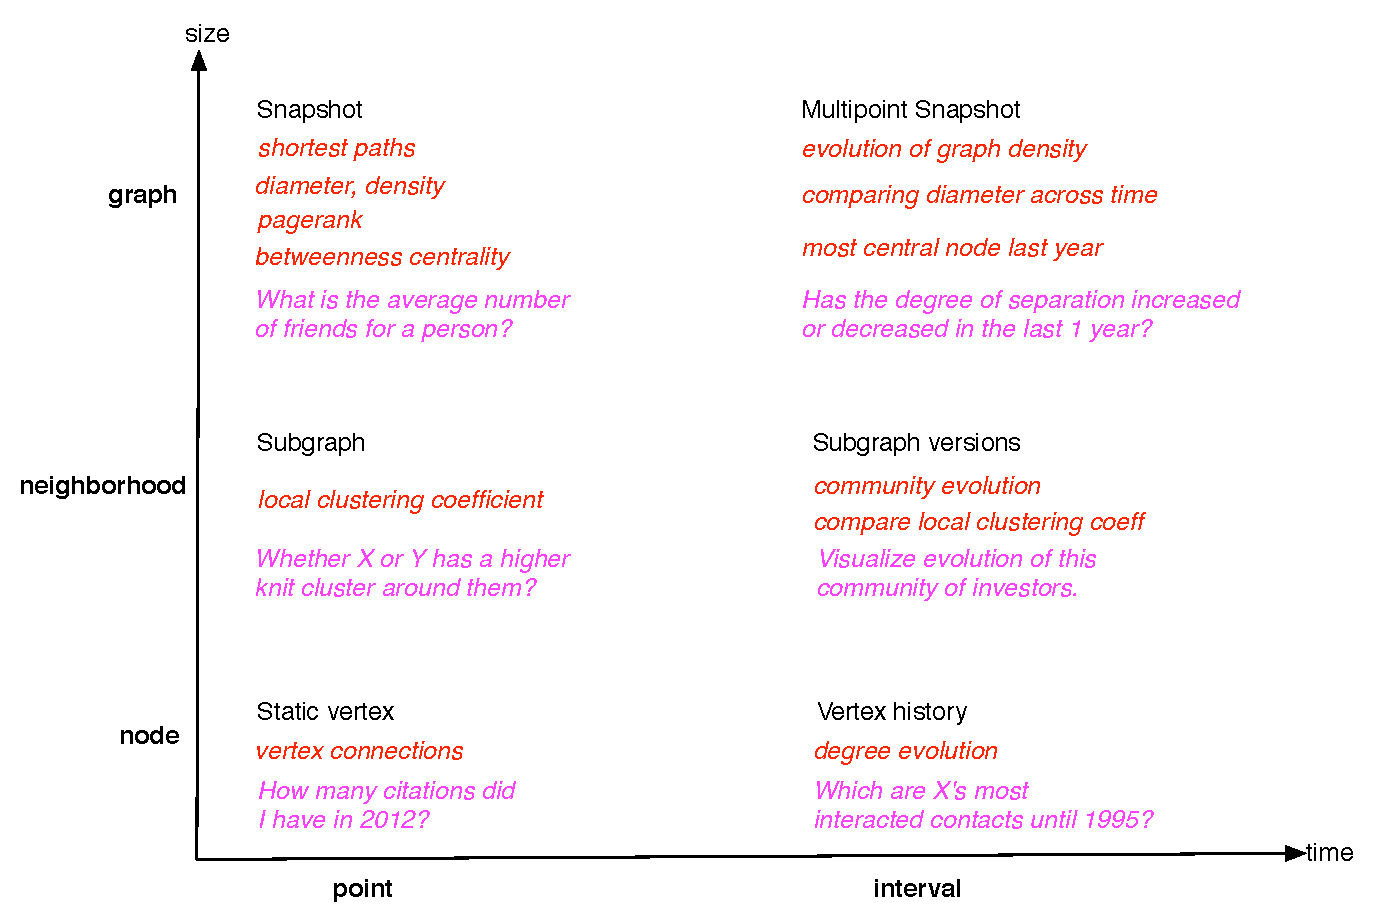
\includegraphics [width=0.75\textwidth]{entity-time.pdf}
\caption{A temporal graph can be represented across two different dimensions - time
and entity. The chart lists retrieval tasks (black), graph operations (red), example queries
(magenta) at different granularities of time and entity size.}
\label{fig:et}
\end{figure}

%Main Text




Broadly speaking, this chapter's focus is to briefly introduce the reader to the recent advances in historical graph data management for temporal graph analytics. 
There are many different types of analyses that may be of interest. 
For example, an analyst may wish to study the evolution of well-studied static graph properties such
as centrality measures, density, conductance, etc., over time; or, the search and 
discovery of temporal patterns, where the events that constitute the pattern are spread out over time. 
Comparative analysis, such as juxtaposition of a statistic over time, or perhaps, computing 
aggregates such as \textit{max} or \textit{mean} over time, gives another style of knowledge discovery 
into temporal graphs. Most of all, even a primitive notion of simply being able to access past states of the graphs 
and performing simple static graph analytics, empowers a data scientist with the capacity to 
perform analysis in arbitrary and unconventional patterns. 
Supporting such a diverse set of temporal analytics and querying over large volumes of historical graph data 
requires addressing several data management challenges. Specifically, we need techniques for storing
the historical information in a compact manner, while allowing a user to retrieve graph snapshots as of any
time point in the past, or the evolution history of a specific node or a specific neighborhood. Further the
data must be stored and queried in a distributed fashion to handle the increasing scale of the data. 
Finally, there is a need for an expressive, high-level, easy-to-use programming framework that will allow users to 
specify complex temporal graph analysis tasks. %, while ensuring that the specified tasks can be executed efficiently 
in a data-parallel fashion across a cluster.

%The purpose of this chapter is to highlight the recent advancements in graph data management system that can efficiently and scalably
%support these types of dynamic network analysis tasks over large volumes of data. 


\section{Storage and Retrieval}

Storage of large temporal graphs is challenging and requires careful design. An effective storage system for temporal graphs has a twofold objective. First, the storage should be compact such that the invariant information across multiple graph versions is not stored multiple times. Second, it must allow for efficient retrieval of graph primitives such as snapshot(s), temporal range queries of nodes or neighborhoods, amongst others, as reflected in Figure~\ref{fig:et}. A straightforward use of static graph datastores can lead to an explosion in storage requirements, and/or incur high fetch latency times.  
Consider two basic and extreme approaches from conventional storage methods 
to support snapshot retrieval queries, referred to as the \textit{Copy} and \textit{Log} approaches, respectively~\cite{Salzberg1999}. While the Copy approach relies on storing new copies of a snapshot upon every point of change, the log approach relies on storing everything through changes. Their hybrid is often referred to as the \textit{Copy+Log} approach. Copy approach is clearly infeasible for frequently changing graphs because of intractable storage needs; the Log approach, while storing minimal information, makes it hard work to reconstruct any snapshot or temporal subset of the graph. %We omit a detailed discussion of the work on temporal databases, and refer the interested reader to a representative set of references~\cite{Bolour92,DBLP:conf/sigmod/SnodgrassA85,Ozsoyoglu1995,Tansel1993,date2002temporal,tsql2,Salzberg1999}. 
%Other data structures, such as Interval Trees~\cite{arge1996optimal} and Segment trees~\cite{Blankenagel1994} can also be used for storing temporal information. 
%Temporal aggregation in scientific array databases~\cite{soroush2013time} and time-series indexing~\cite{niennattrakul2010exact}, ~\cite{camerra2013beyond}, ~\cite{wang2013experimental} are other related topics of interest, but the challenges there are significantly different. In this section, we present some of the most recognized approaches for efficient storage and retrieval of historical graphs.

\subsection{Delta-based Encodings}
The use of ``{\em deltas}'', or graph differences, is a powerful approach to register the changes in a graph over a period of time. If carefully organized, deltas can provide efficient retrieval at low storage costs. 
The {\em DeltaGraph} index~\cite{khurana2013efficient}, for instance, provides highly efficient retrieval of individual snapshots of the historical graph for specific time instances. It organizes the historical graph data in a hierarchical data structure, whose lowest level corresponds
to the snapshots of the network over time, and whose interior nodes correspond to graphs constructed by ``combining''
the lower level snapshots in some fashion; the interior nodes are typically not valid snapshots as of any specific time point. Neither the lowest-level
graph snapshots nor the graphs corresponding to the interior nodes are actually stored explicitly. Instead, for each edge, a {\em delta}, i.e., the
difference between the two graphs corresponding to its endpoints, is computed, and these deltas are explicitly stored. In addition, the graph
corresponding to the root is explicitly stored. Given those, any specific snapshot can be constructed by traversing any
path from the root to the node corresponding to the snapshot in the index, and by appropriately combining the information present in the deltas.
Use of different ``combining'' functions leads to a different point in the performance-storage trade-off, with {\em intersection} being the most
natural such function.  This index structure is especially effective with {\em multi-snapshot retrieval} queries, which are expected to be common in temporal 
analysis, as it can share the computation and retrieval of deltas across the multiple snapshots. 
%The index structure is also {\em extensible}, providing a user the opportunity to define additional 
%indexes to be created and maintained in order to efficiently execute specific queries (e.g., subgraph pattern matching, reachability, etc.) over the historical graph data.
While it is efficient at snapshot retrieval, is not suitable for fetching graph primitives such as histories of nodes or neighborhoods over specified periods of time. However, {\em Temporal Graph Index (TGI)}~\cite{khurana2016storing}, an extension of DeltaGraph which partitions deltas in so-called {\em micro-deltas}, and uses chaining of related microdeltas across horizontal nodes in the DeltaGraph, allows retrieval of different temporal graph primitives including neighborhood versions, node histories, and graph snapshots. 
Such a micro-delta based design is great for distributed storage and parallel retrieval on a cloud. This allows efficient retrieval of not only
entire snapshots, but also of individual neighborhoods or temporal histories of individual neighborhoods.


\subsection{Storing by Time Locality}
Another powerful approach to store and process temporal graphs is based on time-locality. {\em Chronos}~\cite{han2014chronos} targets time-range graph analytics, requiring computation on the sequence of static snapshots of a temporal graph within a time range. An example is, the analysis of change in each vertex's PageRank for a given time range. Obviously, the most straightforward approach of applying computation on each snapshot separately is too expensive. Chronos achieves efficiency by exploiting locality of temporal graphs.
It also leverages the time locality to store temporal graphs on disk in a compact way. The layout is organized in snapshot groups. A snapshot group $G_{t_1,t_2}$ contains the state of $G$ in the time range $[t_1,t_2]$, by including a checkpoint of the snapshot of $G$ at $t_1$ followed by all the updates made till $t_2$. The snapshot group is physically stored as edge files and vertex files in time-locality fashion. For example, an edge file begins with an index to each vertex in the snapshot group, followed by segments of vertex data. The segment of a vertex, in turn, first contains a set of edges associated with the vertex at the start time of the snapshot group, followed by all the edge updates to the vertex. A link structure is further introduced to link edge updates related to the same vertex/edge, so that the state of a vertex/edge at a given time $t$ can be efficiently constructed. %We will revisit time-locality based computation in a later section on temporal graph runtime environments. 

\subsection{Indexing using Multiversion Arrays}
{\em LLAMA}~\cite{macko2015llama} presents an approach where an evolving graph is modeled as a time series of graph snapshots, where each batch of incremental updates produces a new graph snapshot. The graph storage is read-optimized, while the update buffer is write-optimized. 
It augments the compact read-only CSR representation to support mutability and persistence. Specifically, a graph is represented by a single vertex table, and multiple edge tables, one per snapshot. The vertex table is organized as a large multi-versioned array (LLAMA) that uses a software copy-on-write technique for snapshotting, and the record of each vertex $v$ in the vertex table maintains the necessary information to track $v$'s adjacency list from the edge tables across snapshots. 
The array of records is partitioned into equal-sized data pages, and an indirection array is constructed that contains pointers to the data pages. The indirection array fits in L3 cache. To create a new snapshot, the indirection array is copied, with those references to out-dated pages replaced by those to the newly modified pages. Thus, we do not need to copy unmodified pages across snapshots. LAMA stores 16 consecutive snapshots of the vertex table in each file, so that disk space can be easily reclaimed from deleted snapshots. 
The edge table for a snapshot $i$ is organized as a fixed-length array that stores adjacency list fragments consecutively, where each adjacency list fragment contains the edges of a vertex added in snapshot~$i$. An adjacency list fragment of vertex $v$ also stores a continuation record, which points to the next fragment for $v$, or {\em null} if there are no more edges. To support edge deletion, each edge table maintains a deletion vector, which is an array that encodes in which snapshot an edge was deleted.

%Properties on vertices and edges may change and should also support snapshotting. Like the vertex table, each type of property is also stored with a LAMA. Different types of properties are stored in separate LAMAs, so that a job may only load the needed property (or properties) for graph analysis.

%LLAMA buffers incoming updates in a write-optimized lookup table, which stores the newly-added and deleted edges for each vertex. The buffered updates are only written into a new snapshot, and a graph analytics query only runs on the read-optimized graph storage without checking the table of buffered updates.
%LLAMA is a single machine system that stores and incrementally updates an evolving graph in multi-version representation, and it supports both in-memory and out-of-core graph analysis on graph snapshots. LLAMA provides a general-purpose programming model, though vertex-centric or edge-centric computations can be implemented on top of it.

\section{Analytical Frameworks}

Running graph analytics requires dealing with two main aspects -- the runtime system components and the interfaces to express the analytical task. Let us discuss the essentials of both.

\subsection{Runtime Environment Aspects}

\noindent{\bf In-Memory Graph Layouts.} Like the storage and indexing of temporal graphs, dealing with temporal redundancy is important in the in-memory data structures on which analytics are executed. For example, when running a graph algorithm or evaluating a metric on various snapshots of a graph, it might be prohibitively expensive to store all the snapshots in the memory at the same time. However, most graph libraries do require plain isolated version of each graph. The most common solution to this problem is to use an overlaying of multiple versions on one another, and using bitmaps and an additional lookup table to establish the validity of a graph component to one or more versions. This reduces any redundancy of nodes, edges or attributes that occur across multiple versions, yet obtaining access to each snapshot as a static graph through a simple interface. GraphPool~\cite{khurana2013efficient} and Chronos~\cite{han2014chronos} amongst others use variations of this technique. In addition, Chronos also employs such a structure for locality-aware batch scheduling (LABS) of graph computation. More specifically, LABS batches the processing of a vertex across all the snapshots, as well as the information propagation to a neighboring vertex for all the snapshots.

\vspace{2mm}

\noindent{\bf Parallelism.} Temporal graph analytics presents opportunities for parallelization in two different ways. First, evaluating a property across multiple snapshots can be easily parallelized, unless . Second, several static graph computation operations such as Pagerank, can be run in parallel themselves. Determining the optimum level of parallelism for an analytical task can be complex and depends on the exact computation steps, nature of graph data and the resources available. TGAF~\cite{khurana2016storing} provides parallelism by expressing all temporal graphs as RDDs of time evolving nodes or subgraphs and letting the underlying Spark infrastructure plan the parallelism. Leveraging Spark parallelism provides abundant benefits, along with simplicity of design. However, it there are occasions on which certain tasks can be customized for better results. A major drawback with TGAF is the lack of space saving obtained through overlaid structures such as GraphPool. LABS and Llama show effective locality-based multi-core parallelism.%Note that while batch processing such as LABS reduces computation cycles, parallelism becomes more complicated.



%\noindent{\bf In-Memory Graph Layout.} There are two kinds of locality for temporal graphs that can be exploited for efficient data layout: \emph{time} locality, where states of a vertex (or an edge) in consecutive snapshots are stored together; and \emph{structure} locality, where states of neighboring vertices in the same snapshot are laid out close to each other. Due to the complex structure of a graph, structure locality is very hard to achieve. Chronos thus favors time locality for graph layout. The selected snapshots for a temporal graph in a time range are stored together in a vertex data array and an edge array. In the vertex data array, data is grouped by the vertices. The data of a vertex in consecutive snapshots are placed together. In the edge array, all the edges are grouped by the source vertices. Inside each group, every edge stores the target vertex ID and a bitmap indicating the snapshots that contain the edge. 
%Although storing all the snapshots in this aggregate form has some similarity to the aggregate graph concept in TIDE, they are used in different context. TIDE stores sample graphs at the same time point together, whereas Chronos stores snapshots in different time points together.

%\vspace{2mm}

%\noindent{\bf Scheduling of Graph Computation.} To leverage the time-locality graph layout, Chronos employs the locality-aware batch scheduling (LABS) of graph computation. More specifically, LABS batches the processing of a vertex across all the snapshots, as well as the information propagation to a neighboring vertex for all the snapshots. %This batching is similar to the bulk execution model in TIDE, but again TIDE uses it for different sample graphs at the same time point instead of snapshots at different time points. 
%In~\cite{han2014chronos}, the authors show that with a simple partition-by-vertex strategy, LABS significantly improves the performance of graph computation in a multi-core parallel setting.

\vspace{2mm}

\noindent{\bf Incremental Computation.} Time-range graph analysis can benefits from incremental or shared computation. First, for iterative algorithms such as PageRank, if the target time-range contains a sequence of $N$ snapshots $S_0$ to $S_{N-1}$, the result computed on $S_0$ can be used to initialize the solution for $S_1$, and so on until $S_{N-1}$. This reduces the number of iterations needed to converge an algorithm, but also serializes the computations because of the newly created dependence. Chronos utilizes a variation of this principle to effectively perform incremental computation. 
%In the second enhancement, Chronos pre-computes the intersection (or the union) of the $N$ snapshots, applies graph computation on the intersection (or union) graph first, and then uses the final states of this computation as the initial states for all the snapshots and computes all the snapshots in a batch. The second enhancement allows incremental algorithms designed for edge-insertion only to work with temporal graphs with edge deletion.

%\vspace{2mm}



\subsection{Analytical Interfaces}
There are mainly two kinds of historical graph analytical interfaces. The first one, a programmatic interface involves an abstraction of a temporal graph and various operations that can be performed on it, along with calls to several static (sub-)graph routines. The second kind are the visual exploration tools which are usually targeted to more specific types of analytic options but provide an easier means to express the task through GUI interfaces and provide meaningful visualization of the results. One example of a programmatic interface is TGAF~\cite{khurana2016storing}, which abstracts the temporal graph through two main primitives --  {\em Set of temporal nodes (SoN)}, and {\em Set of temporal subgraphs (SoTS)}. The entire temporal graph or any part of it may be expressed as one of these primitives. A SoN is best illustrated as a three dimensional array along the axes of time, nodes and attributes. The system also defines graph manipulation operations such as {\em timeslicing}, {\em selection}, {\em filtering}; compute operators such as {\em node compute map}, {\em temporal node compute map}, {\em node compute delta}, amongst others; it also provides analytical operators such as {\em compare}, {\em evolution}, and such. A rich set of operators enables the expression of complex analytical operations. We omit further details here and refer the interested reader to ~\cite{khurana2016storing} and ~\cite{khurana2015historical}.

Visualization is an effective means for exploring and analyzing a temporal graph. Following is a rather brief and non-exhaustive reference to techniques and tools that have demonstrated such capabilities. 
%Erten et al.~\cite{erten2004exploring} present visual analysis for an evolving dataset in computing literature through properties like diameter, connected components, collaborators, co-authors, topic trends over time.
Using visualization of different snapshots, Toyoda et al.~\cite{toyoda2005system} study events like appearance of pages, relationship between different pages for a historical dataset of Web archive.
%More such examples can be found in a survey by Kerracher et al.~\cite{kerracher2015task}. 
NetEvViz~\cite{khurana2011visual} extends NodeXL (a popular graph analysis tool), to study evolving networks. It uses an edge color coding scheme for comparative study of network growth. Ahn et al.~\cite{ahn2011temporal} focus on different states of graph components in order to visualize temporal dynamics of a social network.
Alternate representations to node-link diagrams have been proposed in order to study temporal nature of social networks, such as TimeMatrix~\cite{yi2010timematrix} that uses a matrix based visualization to better capture temporal aggregations and overlays. A temporal evolution analysis technique based on capturing visual consistency across snapshots can be seen in the work of Xu et al.~\cite{xu2011visualizing}.
A survey by Beck et al.~\cite{beck2014state} lists several other approaches for visual analysis of dynamic graphs. 



\bibliographystyle{alpha}
\bibliography{sample} %for bibtex-example

%For non-Bibtex users:
%\begin{thebibliography}{99}
%\bibitem[Aron 2001]{Aron01} Aron J, Blass B (2001) The future of modern genomics. Blackwell, London
%\bibitem[Brown 2001]{Brown01} Brown B, Aaron M (2001) The politics of nature. In: Smith J (ed) The rise of modern genomics, 3rd edn. Wiley, New York, p 234 -295 
%\bibitem[Smith 1999] {Smith99} Smith J, Jones M Jr, Houghton L et al (1999) Future of health insurance. N Engl J Med 965:325 -329  
%\bibitem[South 1999]{South99} South M (1999) The future of genomics. In: Williams H (ed) Proceedings of the genomic researchers, Boston, 1999
%\end{thebibliography}

\end{document}

